\documentclass[xcolor=dvipsnames,aspectratio=169]{beamer}

% INCLUSIÓN DOS PAQUETES IMPRESCINDIBLES DE IDIOMA E CODIFICACIÓN DE CARACTERE.
\usepackage[T1]{fontenc}
\usepackage[english]{babel}
\usepackage[utf8]{inputenc}
\usepackage{csquotes}

%ACRONYMS para engadir un glosario de acronimos automatizado
% \usepackage[acronyms,nonumberlist,nopostdot,nomain,nogroupskip]{glossaries}
% \input{./acronyms.tex}

% PAQUETES PARA FIGURAS E GRAFICOS
\usepackage{graphicx}
%   \usepackage[pdftex]{graphicx}
  \usepackage{epstopdf}
   \graphicspath{{./img/}}
  % and their extensions so you won't have to specify these with
  % every instance of \includegraphics
   \DeclareGraphicsExtensions{.eps,.pdf,.png,.jpg}   
\usepackage{subfigure}
\usepackage{caption}
\usepackage[inkscapelatex=false]{svg}
\usepackage{ifthen}

%Tikz plots
\usepackage{tikz}
\usepackage{tikzscale}
\usepackage{tikz-dimline}
\usetikzlibrary{plotmarks,patterns,decorations.pathreplacing,backgrounds,calc,arrows,arrows.meta,spy,matrix,backgrounds,shapes,math}

\usepackage{pgfplots}
\pgfplotsset{compat=newest}
\pgfplotsset{plot coordinates/math parser=false}
\usepgfplotslibrary{patchplots,groupplots,fillbetween,polar}
   
% OUTROS PAQUETES DE USO COMUN. HOXE EN DIA OS COMPILADORES SON TAN RAPIDOS QUE EU METO TODOS SEMPRE
% \usepackage{float}
% \usepackage{ucs} 
% \usepackage{subcaption}
\usepackage{psfrag}
\usepackage{verbatim}
\usepackage{amsmath}
\usepackage{amsfonts} 
\usepackage{amssymb} 
\usepackage{amsthm}
\usepackage{pifont}
\usepackage{array}
\usepackage{listings}
\usepackage{stfloats}
\usepackage{algorithm} 
\usepackage{algorithmic} 
\usepackage{url} 
\usepackage{enumerate}
\usepackage{multirow}
\usepackage{wasysym}
\usepackage{cancel}
\usepackage{lmodern}

\usepackage{mathrsfs}  

% DECLARACION DAS FONTES DA UVIGO
\usepackage[sfdefault]{roboto}
\usepackage{librebaskerville}
\setbeamerfont{title}{family=\librebaskerville,size=\Huge}
\setbeamerfont{subtitle}{family=\librebaskerville,size=\large}
% IMPORTANTE: a fonte 'campus' non queda ben para títulos de papers academicos,ç
% pero se de verdade se desexa empregar, seguir os seguintes pasos
% 1) Instalar o comando otftotfm en linux
% 2) sudo otftotfm -a -e texnansx campus_bold.otf CampusBold
% 3) asegurarse que o ficheiro auxiliar ./EETtemplateFiles/fonts/T1CampusBold.df está no directorio de traballo
% 4) descomentar a liña abaixo e comentar a liña que lle asigna librebaskerville arriba
\input{EETtemplateFiles/fonts/T1CampusBold.df}
\setbeamerfont{title}{family=\fontfamily{CampusBold},size=\Huge}

% DETLARACIÓN DO TEMA A USAR
% 
% ESTES TEMAS TEÑEN CABECEIRAS MOI GRANDES
% \usetheme{Berkeley} %large titlebar w/side dossier
% \usetheme{PaloAlto} 
% \usetheme{Copenhagen} %large titlebar w/2 side index
% \usetheme{Antibes} %large titlebar w/tree
% \usetheme{Singapore} %large titlebar w/balls evanescent
% \usetheme{Berlin} %large titlebar w/balls solid
% \usetheme{Dresden} %same as above with different color boxing
% \usetheme{Rochester} %large tittle-only titlebar
% ESTES TEMAS TEÑEN CABECEIRAS MEDIANAS
% \usetheme{CambridgeUS} %title titlebar w/current section
% \usetheme{Malmoe} %title titlebar w/current section Copenhagen style
% \usetheme{Madrid} %title titlebar w/page counter footer
% ESTES TEMAS TEÑEN CABECEIRAS DELGADAS
% \usetheme{Frankfurt} %small titlebar w/ progress balls
% \usetheme{metropolis} %metal
% ESTES TEMAS NON TEÑEN CABECEIRA DE COR, PERO SI TITULO SOBRE BRANCO
% \usetheme{Boadilla} %sombras e decoracion
\usetheme{Pittsburgh} %rectangulos planos
% ESTES TEMAS TEÑEN INDICES OU INFO NUNHA BARRA LATERAL GRANDE
% \usetheme{Goettingen} %right dossier evanescent
% \usetheme{Marburg} %right dossier fading to black
% \usetheme{Bergen} %notebook

%aspect modifiers
\useinnertheme{circles} %this makes item lists nicer
% \useoutertheme{infolines} %toggle thin info borders


% DECLARACIÓN DA COMBINACIÓN DE CORES A USAR. SE NON SE ESPECIFICA NADA TOMA A DEFINIDA POR DEFECTO
\definecolor{EETblue}{HTML}{0094e0} % a mate dark blue
\usecolortheme[named=EETblue]{structure} % EET UVigo blue
% outros temas de cores de beamer
% \usecolortheme{seagull} %makes title boxes gray color with blackr
% \usecolortheme{spruce} %makes title boxes pastel blue - gray color
% cores internos (items)
% \usecolortheme[named=Red]{structure} 
% \usecolortheme[named=Green]{structure} 
% \usecolortheme[named=OliveGreen]{structure} 
% \usecolortheme[named=PineGreen]{structure} 
% \usecolortheme[named=TealBlue]{structure} 
% \usecolortheme[named=SeaGreen]{structure}
% \usecolortheme[RGB={00,78,135}]{structure} % a dark cobalt blue 
% \usecolortheme[RGB={155,0,20}]{structure} % a slighlty darkened mate red

% MODIFICACIONS DAS CORES PARA A PAXINA DE TITULO SIMILAR Á OFICIAL
\setbeamercolor*{title}{use=structure,fg=structure.bg, bg=structure.fg}  
\setbeamercolor*{subtitle}{use=structure,fg=white}  
\setbeamercolor*{author}{use=structure,fg=structure.fg}
% \setbeamercolor*{institute}{use=structure,fg=structure.fg}
\setbeamercolor*{date}{use=structure,fg=structure.fg}
\setbeamertemplate{frametitle}[default][left]

% MODIFICACIONS DA SIDEBAR E FOOTLINE PARA INCLUIR AS IMAXES CORPORATIVAS.
\setbeamertemplate{footline}[text line]{%
  \parbox{\linewidth}{
    %ESTE TEXTO DA FOOTLINE PODESE MODIFICAR A GUSTO -----------------------------------------
    \insertshorttitle\hfill\insertshortauthor\hfill\insertpagenumber / \inserttotalframenumber
    %----------------------------------------------------------------------------------------
    \hfill
  \includegraphics[width=.15\paperwidth,trim={0 2.5cm 3.5cm .75cm},clip]{EETtemplateFiles/img/Logotipo_ESCOLA.pdf}\vspace*{2pt}}}
\setbeamersize{sidebar width left = .10\paperwidth}
\setbeamertemplate{sidebar canvas left}{}
\setbeamertemplate{sidebar left}{%
  \vspace*{\fill}
  \includegraphics[width=.15\paperwidth,height=.15\paperwidth]{EETtemplateFiles/img/Simbolo_ESCOLA.pdf}\\
  \includegraphics[width=.15\paperwidth,trim={.4cm .5cm .4cm 2.25cm},clip]{EETtemplateFiles/img/Logotipo_ESCOLA.pdf}
  \vspace*{-11pt}%
}

% MATH SYMBOLS

\newcommand{\field}[1]{\mathbb{#1}}

\DeclareMathOperator{\atan}{atan}
\DeclareMathOperator{\acos}{acos}
\DeclareMathOperator{\asin}{asin}

% \newcommand{\mb}[1]{\mathbf{#1}}


\newcommand{\Hb}{\mathbf{H}}
\newcommand{\Sb}{\mathbf{\boldsymbol{\Sigma}}}
\newcommand{\Sm}{\mathbf{S}}
\newcommand{\U}{\mathbf{U}}
\newcommand{\F}{\mathbf{F}}
\newcommand{\V}{\mathbf{V}}
\newcommand{\A}{\mathbf{A}}
\newcommand{\B}{\mathbf{B}}
\newcommand{\Cb}{\mathbf{C}}
\newcommand{\D}{\mathbf{D}}
% \newcommand{\E}{\mathbf{E}}
\newcommand{\Gb}{\mathbf{G}}
\newcommand{\T}{\mathbf{T}}
\newcommand{\I}{\mathbf{I}}
\newcommand{\Y}{\mathbf{Y}}
\newcommand{\M}{\mathbf{M}}
\newcommand{\N}{\mathbf{N}}
\newcommand{\W}{\mathbf{W}}
\newcommand{\Z}{\mathbf{Z}}
\newcommand{\R}{\mathbf{R}}
\newcommand{\K}{\mathbf{K}}
\newcommand{\X}{\mathbf{X}}
\newcommand{\Pb}{\mathbf{P}}
\newcommand{\Lb}{\mathbf{L}}
\newcommand{\Phib}{\mathbf{\boldsymbol{\Phi}}}
\newcommand{\Upsb}{\mathbf{\boldsymbol{\Upsilon}}}
\newcommand{\Delb}{\mathbf{\boldsymbol{\Delta}}}
\newcommand{\Xib}{\mathbf{\boldsymbol{\Xi}}}
\newcommand{\Q}{\mathbf{Q}}
% \newcommand{\D}{\mathbf{D}}
\newcommand{\one}{\mathbf{1}}
\newcommand{\zero}{\mathbf{0}}
\newcommand{\Rm}{\mathbf{R^{-1}}}
\newcommand{\LL}{\mathbf{\boldsymbol{\Lambda}}}
\newcommand{\J}{\mathbf{J}}

\newcommand{\ab}{\mathbf{a}}
\newcommand{\bb}{\mathbf{b}}
\newcommand{\cc}{\mathbf{c}}
\newcommand{\dd}{\mathbf{d}}
\newcommand{\e}{\mathbf{e}}
\newcommand{\f}{\mathbf{f}}
\newcommand{\g}{\mathbf{g}}
\newcommand{\h}{\mathbf{h}}
\newcommand{\m}{\mathbf{m}}
\newcommand{\n}{\mathbf{n}}
\newcommand{\pp}{\mathbf{p}}
\newcommand{\q}{\mathbf{q}}
\newcommand{\rr}{\mathbf{r}}
\newcommand{\s}{\mathbf{s}}
\newcommand{\uu}{\mathbf{u}}
\newcommand{\vv}{\mathbf{v}}
\newcommand{\w}{\mathbf{w}}
\newcommand{\x}{\mathbf{x}}
\newcommand{\y}{\mathbf{y}}
\newcommand{\z}{\mathbf{z}}
\newcommand{\al}{\mathbf{\boldsymbol{\alpha}}}
\newcommand{\vmu}{\mathbf{\boldsymbol{\mu}}}
\newcommand{\vlambda}{\mathbf{\boldsymbol{\lambda}}}
\newcommand{\vphi}{\mathbf{\boldsymbol{\phi}}}
\newcommand{\vrho}{\mathbf{\boldsymbol{\rho}}}
\newcommand{\vups}{\mathbf{\boldsymbol{\upsilon}}}

\newcommand{\rank}{\textnormal{rank}}
% \newcommand{\trace}{\textnormal{trace}}
\newcommand{\exptr}{\textnormal{exptr}}
\newcommand{\tr}{\textnormal{tr}}
\newcommand{\vstack}{\textnormal{vec}}
\newcommand{\diag}{\textnormal{diag}}
%  |x>
\newcommand{\ket}[1]{\left\vert#1\right\rangle}
%  <x|
\newcommand{\bra}[1]{\left\langle#1\right\vert}
%  <x|y>
\newcommand{\braket}[2]{\left< #1 \vphantom{#2}\,
                        \right\vert\left.\!\vphantom{#1} #2 \right>}
%  <x|a|y>
\newcommand{\sandwich}[3]{\left< #1 \vphantom{#2 #3} \right|
                          #2 \min\left(\vphantom{#1 #2} #3 \right>}

\newcommand{\pd}[2]{\frac{\partial #1}{\partial #2}}
%  d/dt
\newcommand{\ddt}{\frac{d}{dt}}
%  D/Dx
\newcommand{\pdd}[1]{\frac{\partial}{\partial#1}}
%  |x|
\newcommand{\abs}[1]{\left\vert#1\right\vert}
%  k_{x}
\newcommand{\kv}[1]{\mathbf{k}_{#1}}
%  \textnormal{E}_{domain of integration}{variable}
\newcommand{\Ex}[2]{{\mathbb{E}_{#1}\left[#2\right]}}
\newcommand{\CEx}[3]{{\mathbb{E}_{#1}\left[#2|#3\right]}}
\newcommand{\CInf}[3]{{\textnormal{I}\left(#1;#2|#3\right)}}
\newcommand{\Inf}[2]{{\textnormal{I}\left(#1;#2\right)}}
\newcommand{\CEnt}[2]{{\textnormal{H}\left(#1|#2\right)}}
\newcommand{\Ent}[1]{{\textnormal{H}\left(#1\right)}}
\newcommand{\dCEnt}[2]{{\textnormal{h}\left(#1|#2\right)}}
\newcommand{\dEnt}[1]{{\textnormal{h}\left(#1\right)}}

\newcommand{\cmark}{\ding{51}}%
\newcommand{\xmark}{\ding{55}}%
\newcommand\Tau{\mathcal{T}}
%Figure and format fixes


\renewcommand{\figurename}{Fig.}
\newcommand{\PESrule}{\noindent\rule{.57\columnwidth}{0.1mm}}

% A command to make itemized table contents

%theroem environments
% If using amsthm package, we need to delete these theorems before giving them our own definition. does not work for theorem
% \let\theorem\relax
\let\definition\relax
\let\lemma\relax
\let\corollary\relax
\let\example\relax
%
% \newtheorem{theorem}{Theorem}
\newtheorem{definition}{Definition}
\newtheorem{lemma}{Lemma}
\newtheorem{corollary}{Corollary}
\newtheorem{conjecture}{Conjecture}
\newtheorem{example}{Example}
\theoremstyle{plain}
\newtheorem{remark}{Remark}
\newtheorem{proposition}{Proposition}
   \newtheorem{homework}{Homework}

%Colors
   \definecolor{blueH3}{rgb}{0,.5,1}
   \definecolor{blueH2}{rgb}{0,0.25,0.75}
   \definecolor{blueH1}{rgb}{0,0,0.5}   
   \definecolor{grayOldText}{rgb}{.5,.5,.5}
   \definecolor{VCobalt}{HTML}{005682}
   \definecolor{TZTeal}{HTML}{008080}
   \definecolor{TZTealfaded}{HTML}{F0FFFF}
   \definecolor{KYJade}{HTML}{008151}
   \definecolor{ARust}{HTML}{a10000}
   \definecolor{FFucsia}{HTML}{7000c3}   
   \definecolor{TAMustard}{HTML}{a1a100}
   \definecolor{Tangerine}{HTML}{d45500}
   
   
  \newcommand{\itempro}{\item[\textcolor{KYJade}{\Large \cmark}]}
  \newcommand{\itemcontra}{\item[\textcolor{ARust}{\Large \xmark}]}
   
   %%%%%%%%%%%%%%%%%%%%%%%%%%%%%%%%%%%%%%%%%%%%%%%%%%%%%%%%%%%%%%%%%
%% The following definitions are to extend the LaTeX algorithmic 
%% package with SWITCH statements and one-line structures.
%% The extension is by 
%%   Prof. Farn Wang 
%%   Dept. of Electrical Engineering, 
%%   National Taiwan University. 
%% 
\newcommand{\SWITCH}[1]{\STATE \textbf{switch} (#1)}
\newcommand{\ENDSWITCH}{\STATE \textbf{end switch}}
\newcommand{\CASE}[1]{\STATE \textbf{case} #1\textbf{:} \begin{ALC@g}}
\newcommand{\ENDCASE}{\end{ALC@g}}
\newcommand{\CASELINE}[1]{\STATE \textbf{case} #1\textbf{:} }
\newcommand{\DEFAULT}{\STATE \textbf{default:} \begin{ALC@g}}
\newcommand{\ENDDEFAULT}{\end{ALC@g}}
\newcommand{\DEFAULTLINE}[1]{\STATE \textbf{default:} }
%% 
%% End of the LaTeX algorithmic package extension.

\newcounter{MYtempeqncnt}


%%%%%%%%%%%%%%%%%%%%%%%%%%%%%%%%%%%%%%%
% Commands to recall text later
%%%%%%%%%%%%%%%%%%%%%%%%%%%%%%%%%%%%%%%
\makeatletter
\newcommand\remembertext[2]{% #1 is a key, #2 is the text
  \immediate\write\@auxout{\unexpanded{\global\long\@namedef{mytext@#1}{#2}}}%
  #2%
}
%
\newcommand\recalltext[1]{%
  \ifcsname mytext@#1\endcsname
    \@nameuse{mytext@#1}%
  \else
    ``??''
  \fi
}

%%%%%%%%%%%%%%%%%%%%%%%%%%%%%%%%%%%%%%%%%%%%%%%%%%%%%%%%%%%%%%%%%%%%%%%%%%%%%%%%%%
%%% Paolo Casari: macros for automating section titling and comment formatting %%%
%%%%%%%%%%%%%%%%%%%%%%%%%%%%%%%%%%%%%%%%%%%%%%%%%%%%%%%%%%%%%%%%%%%%%%%%%%%%%%%%%%
\newcounter{myequationcnt}

\newcounter{rcnt}
\newcounter{ccnt}

\newcommand{\newreviewernopagebreak}[1]{\vspace{5em} \setcounter{ccnt}{0}\section*{\normalsize Comments of #1}\vspace{4mm}}

\newcommand{\ThisIsTheEditorNoPageBreak}{\setcounter{ccnt}{0}\section*{\Large Comments of the Editor}\vspace{3mm}}
\newcommand{\ThisIsTheEditor}{\clearpage \ThisIsTheEditorNoPageBreak}
\newcommand{\ThisIsANewReviewerNoPageBreak}[1]{\vspace{5em} \refstepcounter{rcnt}\label{r#1}\setcounter{ccnt}{0}\section*{\Large Comments of Reviewer \arabic{rcnt}}\vspace{3mm}}
\newcommand{\ThisIsANewReviewer}[1]{\clearpage\vspace{-5em} \ThisIsANewReviewerNoPageBreak{#1}}

\newcommand{\edcomment}[1]{
\begin{tcbremark}
\color{VCobalt}
    \refstepcounter{ccnt}\label{e\arabic{ccnt}}\noindent\textbf{\boldmath\emph{Comment E.\arabic{ccnt}:}} #1\vspace{0.2cm}
\end{tcbremark}
}
\newcommand{\refedcomment}[1]{E.\ref{e#1}}

\newcommand{\revcomment}[1]{
\begin{tcbremark}
\color{VCobalt}
\refstepcounter{ccnt}\label{r\arabic{rcnt}c\arabic{ccnt}}\noindent\textbf{\boldmath\emph{Comment \arabic{rcnt}.\arabic{ccnt}:}} #1\vspace{0.2cm}
\end{tcbremark}
}
\newcommand{\refrevcomment}[2]{\ref{r#1}.\ref{r#1c#2}}

% \newcommand{\ouranswer}[1]{\noindent\emph{Answer:} #1\vspace{0.6cm}}
% \newcommand{\citepap}[1]{\vspace{0.33cm}\begin{minipage}{0.05\textwidth} $\phantom{A}$  \end{minipage}\begin{minipage}{0.85\textwidth}\renewcommand{\baselinestretch}{1.15}\small \emph{#1} \end{minipage}\vspace{0.3cm}}

\newlength{\ansspace}
\addtolength{\ansspace}{0.6cm}
\newcommand{\ansbreak}{\vspace{\ansspace}}

\newlength{\stdleftskip}
\addtolength{\stdleftskip}{\leftskip}
\newlength{\stdrightskip}
\addtolength{\stdrightskip}{\rightskip}
\newlength{\citeskip}
\addtolength{\citeskip}{2em}
\newcommand{\oldbaselinestretch}{1.5}

\newcommand{\setcitepapskip}{%
    \leftskip\citeskip %
    \rightskip\citeskip %
    \renewcommand{\baselinestretch}{1.15}\small%
    \vspace{0.6em}%
    \noindent%
}

\newcommand{\resetLRmargins}{%
    \leftskip\stdleftskip %
    \rightskip\stdrightskip %
    \renewcommand{\baselinestretch}{\oldbaselinestretch}\normalsize %
    \vspace{0.6em}
}

\newcommand{\emans}{\emph{Answer:\ }}


%---------------
% LIMIAR
%---------------
%configuracion de opcions de beamer persoais, pero alleas ao estilo

% COMANDO QUE INTRODUCE UNHA DIAPOSITIVA CUN ÍNDICE NO QUE APARECEN VELADAS TÓDALAS SECCIÓNS MENOS A ACTUAL. ÚTIL PARA INTRODUCIR OS TÍPICOS ÍNDICES INTERMEDIOS.
\newcommand{\Inter}{\frame{\tableofcontents[currentsection]}}
\newcommand{\inter}{\frame{\tableofcontents[currentsection,currentsubsection]}}

% Pes de imaxe
\renewcommand{\figurename}{Fig.}
\addto\captionsenglish{\renewcommand{\figurename}{Fig.}}
\setbeamertemplate{caption}[numbered]

%ESTE PAQUETE PERMITE POÑER A BIBLIOGRAFIA AO PE DE PAXINA CON CONFIGURACIONS ESTETICAS PERSOAIS
% \usepackage[style=ieee,doi=false,isbn=false,url=true,backend=bibtex]{biblatex}
% \bibliography{./bibliografia.bib}
% \newrobustcmd*{\footfullcitenomark}{%
%   \AtNextCite{%
%     \let\thefootnote\relax 
%     \let\mkbibfootnote\mkbibfootnotetext
%     }%
%   \footfullcite}

%paquete para engadir notas de guion ao pdf
\usepackage{pgfpages}
% \setbeameroption{show only notes} 
% \setbeameroption{show notes}
% \setbeameroption{show notes on second screen=right}
% DATOS DO DOCUMENTO
\title[CDA]{Advanced Digital Communications}
\subtitle{Session 6: Advanced Multicarrier Designs}
\author[FGC]{\underline{Felipe G\'omez-Cuba}}
\institute[GPSC]{
\begin{columns}[T]
\begin{column}{5cm}\centering
Office A-204\\
Wednesday \& Thursday 15:00-18:00\\
\texttt{gomezcuba@gts.uvigo.es}\\
\end{column}
\end{columns}
}

\date{2025}


\begin{document}

% Diapositiva co título
\frame[plain]{\titlepage}

\frame{

\frametitle{Orthogonal Frequency Division Multiplexing (OFDM)}
 \begin{figure} 
 \centering
 \caption{1G $\to$ 4G: New standard $\equiv$ new modulation waveform}
 \subfigure[3GPP Standards]{
    \includegraphics[width=.4\columnwidth]{generations}
 }
 \subfigure[WiFi Standards]{
   \scalebox{.45}{
    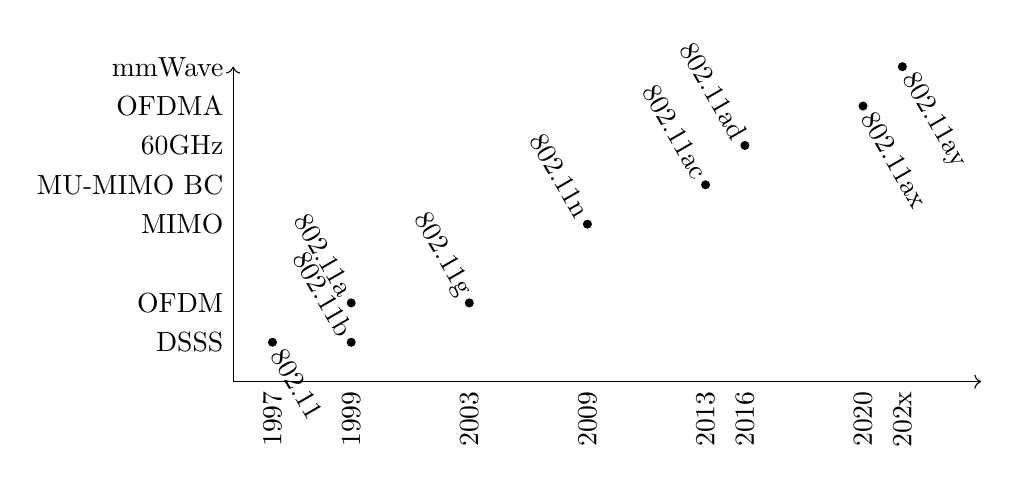
\begin{tikzpicture}
    \draw[->] (0,0) -- (9.5,0);
    \draw[->] (0,0) -- (0,4);
    
    \node[anchor=east, rotate=90] at (.5,0) {1997};
    \node[anchor=east] at (0,.5) {DSSS};
    
    \node[draw,circle,fill=black,inner sep=1] at (.5,.5) {};
    \node[anchor=west,rotate=-60] at (.5,.5) {802.11};
    
    \node[anchor=east, rotate=90] at (1.5,0) {1999};
    \node[draw,circle,fill=black,inner sep=1] at (1.5,.5) {};
    \node[anchor=east, rotate=-60] at (1.5,.5) {802.11b};
    
    \node[anchor=east] at (0,1) {OFDM};
    \node[draw,circle,fill=black,inner sep=1] at (1.5,1) {};
    \node[anchor=east, rotate=-60] at (1.5,1) {802.11a};
    
    \node[anchor=east, rotate=90] at (3,0) {2003};
    \node[draw,circle,fill=black,inner sep=1] at (3,1) {};
    \node[anchor=east, rotate=-60] at (3,1) {802.11g};
    
    \node[anchor=east] at (0,2) {MIMO};
    \node[anchor=east, rotate=90] at (4.5,0) {2009};
    \node[draw,circle,fill=black,inner sep=1] at (4.5,2) {};
    \node[anchor=east, rotate=-60] at (4.5,2) {802.11n};
    
    \node[anchor=east, rotate=90] at (6,0) {2013};
    \node[anchor=east] at (0,2.5) {MU-MIMO BC};
    \node[draw,circle,fill=black,inner sep=1] at (6,2.5) {};
    \node[anchor=east, rotate=-60] at (6,2.5) {802.11ac};
    
    \node[anchor=east, rotate=90] at (6.5,0) {2016};
    \node[anchor=east] at (0,3) {60GHz};
    \node[draw,circle,fill=black,inner sep=1] at (6.5,3) {};
    \node[anchor=east, rotate=-60] at (6.5,3) {802.11ad};
    
    \node[anchor=east, rotate=90] at (8,0) {2020};
    \node[anchor=east] at (0,3.5) {OFDMA};
    \node[draw,circle,fill=black,inner sep=1] at (8,3.5) {};
    \node[anchor=west, rotate=-60] at (8,3.5) {802.11ax};
    
    \node[anchor=east, rotate=90] at (8.5,0) {202x};
    \node[anchor=east] at (0,4) {mmWave};
    \node[draw,circle,fill=black,inner sep=1] at (8.5,4) {};
    \node[anchor=west, rotate=-60] at (8.5,4) {802.11ay}; 
    \end{tikzpicture}
   }
  }
\end{figure}    

\begin{itemize}
\begin{columns}[T]
 \begin{column}{7cm}
 \item New 5G waveforms were proposed
 \begin{itemize}
    \itemcontra Cyclic prefix
    \itemcontra Peak-to-average-power-ratio (PAPR) 
    \itemcontra Synchronization (time \& frequency)
    \itemcontra Spectrum sidelobes
    \end{itemize}
 \end{column} 
 \begin{column}{6cm}
 \item OFDM prevails in 5G and WiFi 7
 \begin{itemize}
    \itempro Simple DFT channel equalizer 
    \itempro Versatile OFDMA scheduling (Everything over-the-top of IP)
    \end{itemize}
 \end{column} 
\end{columns}
\end{itemize}
}


\frame[allowframebreaks]{
\frametitle{Review of OFDM}
\begin{columns}
 \begin{column}{6cm}
\begin{itemize}
\item Transmitted RF real signal
    \begin{eqnarray}
    \nonumber
    x(t)=\sqrt{2} \Re \{s(t) e^{j2\pi f_c t}\}
    \end{eqnarray}
\item Baseband complex signal
\begin{eqnarray}
\nonumber
\label{eq:OFDM_vec}
s(t)=\sum_{n} \sum_{k=0}^{K-1} A_k [n] \textcolor{VCobalt}{\phi_k (t-nT)}
\end{eqnarray}
\item Orthonormal basis pulses
\begin{eqnarray}
\label{eq:forma_phi_l}
\nonumber
\textcolor{VCobalt}{\phi_k(t)}=\textcolor{TZTeal}{e^{-j\frac{2 \pi k t}{T}}}\cdot{}\textcolor{TAMustard}{w_T(t)}
\end{eqnarray}
\item Rectangular time window
\begin{eqnarray}
\nonumber
\textcolor{TAMustard}{w_T(t)}=  \begin{cases}
    1 & 0 \leq t < T\\
    0 & \text{otherwise}
  \end{cases} 
\end{eqnarray}
\end{itemize}
 \end{column}
 \begin{column}{6cm}
 \begin{figure}
  \centering
%   \caption{} 
\subfigure[$\phi_3(t)$]{
        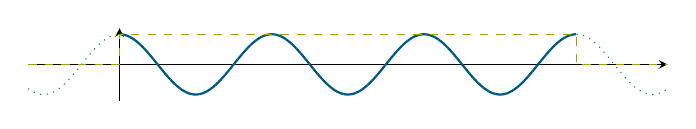
\begin{tikzpicture}
        \begin{axis}[ymax=1,ymin=-1,xmin=-2,xmax=12,height=2.5cm,width=.8\columnwidth,    
        ticks=none,
        axis x line=middle,
        axis y line=middle,
        enlarge y limits=true]
        \addplot[VCobalt,thick,domain=0:10,samples=200] { cos(360*x*3/10)};
        \addplot[dotted,TZTeal,domain=-2:12,samples=200] { cos(360*x*3/10)};
        \addplot[dashed,TAMustard,domain=-2:12,samples=200] coordinates{
        (-2,0)
        (0,0)
        (0,1)
        (10,1)
        (10,0)
        (12,0)};
        \end{axis}
        \end{tikzpicture}
    }
\subfigure[$\phi_2(t)$]{
        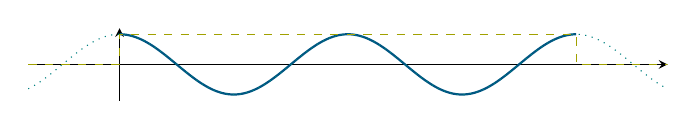
\begin{tikzpicture}
        \begin{axis}[ymax=1,ymin=-1,xmin=-2,xmax=12,height=2.5cm,width=.8\columnwidth,    
        ticks=none,
        axis x line=middle,
        axis y line=middle,
        enlarge y limits=true]
        \addplot[VCobalt,thick,domain=0:10,samples=200] { cos(360*x/5)};
        \addplot[dotted,TZTeal,domain=-2:12,samples=200] { cos(360*x/5)};
        \addplot[dashed,TAMustard,domain=-2:12,samples=200] coordinates{
        (-2,0)
        (0,0)
        (0,1)
        (10,1)
        (10,0)
        (12,0)};
        \end{axis}
        \end{tikzpicture}
    }
\subfigure[$\phi_1(t)$]{
        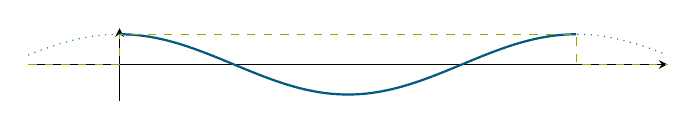
\begin{tikzpicture}
        \begin{axis}[ymax=1,ymin=-1,xmin=-2,xmax=12,height=2.5cm,width=.8\columnwidth,    
        ticks=none,
        axis x line=middle,
        axis y line=middle,
        enlarge y limits=true]
        \addplot[VCobalt,thick,domain=0:10,samples=200] { cos(360*x/10)};
        \addplot[dotted,TZTeal,domain=-2:12,samples=200] { cos(360*x/10)};
        \addplot[dashed,TAMustard,domain=-2:12,samples=200] coordinates{
        (-2,0)
        (0,0)
        (0,1)
        (10,1)
        (10,0)
        (12,0)};
        \end{axis}
        \end{tikzpicture}
    }
\subfigure[$\phi_0(t)$]{
        \begin{tikzpicture}
        \begin{axis}[ymax=1,ymin=-1,xmin=-2,xmax=12,height=2.5cm,width=.8\columnwidth,    
        ticks=none,
        axis x line=middle,
        axis y line=middle,
        enlarge y limits=true]
        \addplot[VCobalt,thick,domain=0:10,samples=200] { cos(0)};
        \addplot[dotted,TZTeal,domain=-2:12,samples=200] { cos(0)};
        \addplot[dashed,TAMustard,domain=-2:12,samples=200] coordinates{
        (-2,0)
        (0,0)
        (0,1)
        (10,1)
        (10,0)
        (12,0)};
        \end{axis}
        \end{tikzpicture}
    }
 \end{figure}
 \end{column}
\end{columns}

\pagebreak

\begin{figure}
 \centering
 \caption{Continuous-time OFDM (we study this for simpler notation)}
  \subfigure[Transmitter]{
  \includegraphics[width=.4\columnwidth]{FDM_mod.png}
  }
  \subfigure[Receiver]{
  \includegraphics[width=.4\columnwidth]{FDM_demod.png}
  }
\end{figure}
\vspace{-.2in}
\begin{figure}
 \centering
 \caption{Discrete time OFDM / DMT (sampling $s[m]=s(m T_s)$, interpolation $g(t)$)}
  \subfigure[Transmitter]{
  \includegraphics[width=.4\columnwidth]{FDM_dft.png}
  }
  \subfigure[Receiver]{
  \includegraphics[width=.4\columnwidth]{demod2_disc.png}
  }
\end{figure}
}

\frame{
\frametitle{The problem of Synchronization}
\begin{theorem}[No ISI/ICI]
Orthonormal Pulses
$$\braket{\boldsymbol{\phi}_k(t)}{\boldsymbol{\phi}_\ell(t)}  =  
\int_{0}^T e^{\frac{j 2 \pi k t}{T}} e^{-j\frac{2 \pi \ell t}{T}} dt = T \delta [k-\ell]\;\forall k,\ell \in \{0, \cdots, K-1 \}$$
Ideal channel output $q[k]=A[k]+\sum_{l\neq k}A[\ell]\textcolor{ARust}{\cancel{\braket{\boldsymbol{\phi}_k(t)}{\boldsymbol{\phi}_l(t)}}}+z[k]$
\end{theorem}
% \begin{proof}
 \begin{itemize}
 \item Requires pulses aligned in time
 \item Requires frequencies exact multiple of $2\pi/T$
\end{itemize}
% \end{proof}
\begin{definition}[\textcolor{ARust}{Synchronization ICI/ISI}]
When multiple transmitters use different oscillator or clock. Such as multiple BSs in cooperation, or specially multiple mobiles in uplink!!
\end{definition}
}

\frame{
\frametitle{The problem of Side Lobes}
\begin{itemize}
\item Rectangular Window
$$\phi_k(t)=e^{-j\frac{2 \pi k t}{T}}\cdot{}w_T(t)\; \stackrel{\mathcal{FT}}{\longleftrightarrow}\; \Phi_k(f)=\delta(f-k\Delta f)*\textnormal{sinc}(\frac{f}{\Delta f})\textnormal{ with }\Delta f=1/T$$
\item Undesired levels of side lobes. 
\end{itemize}
\begin{figure}
\centering
 \subfigure[$|\Phi_k(f)|^2$]{\includegraphics[width=.45\textwidth]{phi9.png}}
 \subfigure[$|S(f)|^2$]{\includegraphics[width=.45\textwidth]{completo4.png}}
\end{figure}
}

\frame[allowframebreaks]{
\frametitle{Filtered OFDM}
\begin{definition}[Biorthogonality]
 \begin{itemize}
 \item Received pulses $\psi_k(t)$ different from the transmitted pulses $\phi_k(t)$
 \item \textit{Generalized Nyquist criterion}
    \begin{equation*}
    \braket{\phi_k(t-mT)}{\psi_l (t-nT)} = \int_{-\infty}^\infty \phi_k(t-mT) \psi^*_l (t-nT) dt = \delta[k-l] \delta[m-n]
    \end{equation*}
 \item Simplifies to Nyquist criterion with only one pulse $k=l$
 \end{itemize}
\end{definition}
\begin{example}[Cyclic Prefix OFDM (CP-OFDM)]
\begin{equation*}
\phi_k(t)=e^{-j 2 \pi \delta f k t}\cdot{}w_{T}(t)\qquad \psi_l (t)=e^{-j 2 \pi \delta f l t}\cdot{}w_{T_{\text{FFT}}}(t)
\end{equation*}
where $T=T_{CP}+T_{FFT}$ and $\Delta f=\frac{1}{T_{FFT}}$
\end{example}
\pagebreak

\begin{figure}
 \centering
 \caption{Time-Frequency Lattice}
 \includegraphics[width=0.5\textwidth]{time-frequency-lattice.png}
\end{figure}
\begin{itemize}
\item 2D grid of subcarriers (frequency) and OFDM symbols (time)
\item Symbol density $\Delta f \cdot T \geq 1$
\begin{itemize}
\item Equality achieved only by giving up orthogonality
\end{itemize}
\end{itemize}
\pagebreak

\begin{itemize}
\item Sharp rectangular $w_T(t)\to$ $\mathrm{sinc}(\frac{f}{\Delta f})\to$ large sidelobes\\ \ \\
\item Design windows $w_T(t)$ with smoother transitions
\end{itemize}
\begin{columns}
 \begin{column}{6cm}
\begin{figure}
 \centering
 \caption{\textit{Raised-Cosine} window}
 \includegraphics[width=0.9\textwidth]{rcresponse.png} 
\end{figure}
 \end{column}
 \begin{column}{6cm}
    \begin{itemize}
    \item This case RC in time (typically RC in frequency)\\ \ \\
    \item Transmission time overlap $T_0$ between adjacent symbol periods \\ \ \\
    \item Reception roll-off time is $T_1$
\end{itemize}
 \end{column}
\end{columns}


\begin{figure}
 \centering
 \caption{\textit{Raised-Cosine} viewed as rectangle $*$ sinusoid fragment}
 \includegraphics[width=1\textwidth]{rcresponse2.png}
\end{figure}
\begin{itemize}
\item $\mathcal{FT}\to$ sinc (big sidelobes) $\times$ shaping filter $H(j\omega)$
\begin{columns}
 \begin{column}{6cm}
\item $T_0 < T\to$ shape of $H(j\omega)$ has
\begin{itemize}
    \itemcontra Wider main lobe than sinc
    \itempro Suppression of sidelobes
\end{itemize}
 \end{column}
 \begin{column}{6cm}
\item Beyond RC windows: 
\begin{itemize}
    \item Filters $H(j\omega)$ design trade-off
    \item Optimal$\to$ \textit{prolate function}
\end{itemize}
 \end{column}
\end{columns}

\end{itemize}
\begin{figure}
 \centering
 \caption{Multiple Window Design Strategies}
 \includegraphics[width=.9\textwidth]{window-designs.png}
\end{figure}
}
% 
% \frame[allowframebreaks]{
% \frametitle{Ambiguity function}
% \begin{itemize}
% \item Window limited to one symbol period
% \begin{itemize}
% \item Time localization $\leftrightarrow$ frequency spreading
% \item Better designs following generalized Nyquist criterion
% \end{itemize}
% \end{itemize}
% \begin{definition}[Ambiguity Function]
%     \begin{equation*}
%         A_{\psi,\phi}(\tau,\nu)=\int_{-\infty}^\infty \psi_l(t) \phi_k^*(t-\tau) e^{-j 2\pi \nu t} dt
%     \end{equation*} 
% \end{definition}
% \begin{theorem}[Generalized Nyquist Criterion vs Ambiguity Function]
% \begin{equation*}
% \braket{ \phi_k(t-mT)}{\psi_l (t-nT)} = A_{\psi,\phi} ((n-m)T,(l-k) \Delta f) = \delta[n-m] \delta[l-k]
% \end{equation*}
% \end{theorem}
% 
% \begin{columns}
%  \begin{column}{6cm}
%     \begin{figure}
%     \centering
%     \caption{Ambiguity Funciton for RC prototype filter (in frequency!)}
%     \includegraphics[width=0.85\columnwidth]{rc-ambiguity.png}
%     \end{figure}
%  \begin{itemize}
% \item Example roll-off $\alpha=0.5$
% \end{itemize}
% \begin{equation*}
%     w_T(t) = \frac{\sin \left( \frac{(1-\alpha) \pi t}{T} \right) + \frac{4 \alpha t}{T} \cos \left(  \frac{(1+\alpha)\pi t}{T} \right)}{\frac{\pi t}{T} \left( 1- \left(\frac{4 \alpha t}{T} \right)^2 \right)}
% \end{equation*}
%  \end{column}
%  \begin{column}{7cm}
%  \begin{itemize}
% \item $\nu \in [-(1+\alpha)/T, (1+\alpha)/T]$\\ \ \\
% \item Infinite time response ($\tau$)\\ \ \\
% \item Safe to sample at zeros of $A(\tau,\nu)$
%     \begin{itemize}
%     \itempro For $\nu=0$, $\tau= \pm T, \pm 2T, \cdots$\\ \ \\
%     \end{itemize}
% \item Imperfect synchronization
%     \begin{itemize}
%         \itemcontra sampling outside zeros\\ \ \\
%     \end{itemize}
%  \item Time-frequency dispersive channel
%     \begin{itemize}
%         \itemcontra Ambiguity function blurred
%     \end{itemize}
% \end{itemize}
%  \end{column}
% \end{columns}
% }
% 
% 
\frame[allowframebreaks]{
\frametitle{Filter Bank Multicarrier}
\begin{columns}
 \begin{column}{5.5cm}
    \begin{figure}
    \centering
    \caption{Time-frequency lattice for RC pulse with density $T\cdot \Delta f = (1+\alpha)$}
    \includegraphics[width=0.9\columnwidth]{rc-grid.png}
    \end{figure}
 \end{column}
 \begin{column}{7cm}
\begin{itemize}
\item One separate filter for each carrier
    \begin{itemize}
        \itemcontra Large hardware Complexity\\ \ \\
    \end{itemize}
\item Better prototype filters
    \begin{itemize}
        \itempro Better time and frequency localization
        \itemcontra Difficult
    \end{itemize}
\end{itemize}
 \end{column}
\end{columns}
}
% \pagebreak
% 
% \begin{definition}[dispersion]
% \begin{equation*}
% \sigma_\tau = \sqrt{\int_{-\infty}^\infty t^2 |p_T(t)|^2 dt}; \ \  \sigma_\nu = \sqrt{\int_{-\infty}^\infty f^2 |p_T(f)|^2 df}
% \end{equation*}
% \end{definition}
% \begin{theorem}[Heinsenberg's uncertainty principle]
%  $$\sigma_\tau \sigma_\nu \geq 1/(4\pi)$$
%  \end{theorem}
% 
%  \begin{itemize}
% \item Equality achieved with (and only with) Gaussian pulse
%     \begin{itemize}
%         \itemcontra Do not satisfy generalized Nyquist criterion\\ \ \\
%     \end{itemize}
% \item {\em Isotropic orthogonal transform algorithm} (IOTA)
%     \begin{itemize}
%         \itempro Prototype filters approaching Heisenberg's limit
%         \itempro Satisfy generalized Nyquist criterion
%     \end{itemize}
% \end{itemize}
% } 
% 
% \frame[allowframebreaks]{
% \frametitle{OFDM-OQAM}
% \begin{itemize}
% \item {\em Offset QAM} OFDM using real constellations ($A_k[n]\in\mathbb{R}$)
% \begin{equation*}
% s(t)=\sum_{n} \sum_{k=0}^{N-1} \textcolor{KYJade}{j^{n+k}} A_k [n] p_T(t-nT\textcolor{KYJade}{/2}) e^{j 2\pi k/T}
% \end{equation*}
% \begin{columns}[T]
%  \begin{column}{9cm}
%     \item Even $n$ $\to$ 
%     \begin{itemize}
%         \item Even carriers $k$ purely real ($j^{2}\cdot A_k[n]$)
%         \item Odd carriers purely imaginary ($j \cdot A_k[n]$)
%     \end{itemize}
%  \end{column}
%  \begin{column}{4cm}
%     \item Odd $n$ $\to$ reverse
%  \end{column}
% \end{columns}
% \pagebreak
% \item Equivalent 'staggered' periods
% \begin{equation*}
% s(t)=\sum_{n} \sum_{k=0}^{N-1} A^e_k [n]  \phi_k^e(t-nT)+\sum_{n} \sum_{k=0}^{N-1} A^o_k [n]  
% \phi_k^o(t-nT-T/2)
% \end{equation*}
% \item Equivalent symbols $A^e_k$ and $A^o_k$\\ \ \\
% 
% \item Receive filters $\phi^e_l(t-mT)$ and $\phi_l^o(t-mT-T/2)$ and taking the {\em real part}, where
% \begin{equation*}
% \phi_k^e(t) = j^k p_T(t) e^{j 2 \pi k t/T}, \ \ \phi_k^o(t)=j \cdot j^{k} p_T(t) e^{j 2 \pi k t/T}
% \end{equation*} 
% 
% \pagebreak
% 
% \item Generalized Nyquist condition for $\phi^e_k(t)$ vs $\phi^e_l(t)$ and $\phi^o_k(t)$ vs $\phi^o_l(t)$\\ \ \\
% \item But we require cross-terms too
% \begin{equation*}
% \Re\left\{\braket{ \phi^e_k(t-mT) }{ \phi^o_l (t-nT-T/2) } \right\}= 0
% \end{equation*}  
% \begin{theorem}[Conventional OFDM pulses satisfy this]
% \begin{equation*}
% \langle \phi_k^e(t), \phi_l^o(t-T/2) \rangle_{\mathbb R}  =  {\text {Re}} \left\{  j^{k-l+1}\int_{T/2}^T \cos (2\pi (k-l)/T) + j \sin (2\pi (k-l)/T) dt \right\} =0
% \end{equation*}
% \begin{itemize}
%     \item Cosine integral always zero
%     \item Sine integral non-zero only if $k-l$ odd $\to$ purely imaginary
%     \item For $k=l$ also purely imaginary
% \end{itemize}
% \end{theorem}
% \end{itemize}
% 
% \pagebreak
% \begin{columns}
%  \begin{column}{7cm}
% \begin{itemize}
% \item Two overlapped modulations $\to$
% \begin{itemize}
% \itemcontra Symbols real, no rate advantage\\ \ \\
% \end{itemize}
% \item $w_T(t)$ even symmetry $\to$
% \begin{itemize}
% \itempro  no even$\leftrightarrow$odd carrier interference
% \itempro  twice grid density\\ \ \\
% \end{itemize}
% \item More efficient joint FBMC-OQAM method also possible
% \end{itemize}
%  \end{column}
%  \begin{column}{6cm}
%   \begin{figure}
%    \centering
%    \includegraphics[width=.8\columnwidth]{OQAM-grid.png}
%   \end{figure}
%  \end{column}
% \end{columns}
% }

\frame{
\frametitle{Universal Filtered Multicarrier (UFMC)}
\begin{itemize}
\item Time-filtered OFDM: All carriers filtered simultaneously
\begin{itemize}
\itemcontra One-symbol localization with extended window $T(1+\alpha)$
\itempro Simple shaping filter (all subcarriers, zeros $\frac{1}{T}$)
\end{itemize}
\item FBMC: requires one filter per each carrier
\begin{itemize}
\itempro Multi-symbol localization with zero interval $T$
\itemcontra Complex subcarrier filter (expanded subcarrier separation $\frac{1}{T}(1+\alpha)$)
\end{itemize}
\item UFMC: filter subbands formed by groups of carriers
\begin{itemize}
\item Trade-off between localization and complexity
\end{itemize}
\end{itemize}
  \begin{figure}
   \centering\includegraphics[width=0.7\textwidth]{UFMC.png}
  \end{figure}
}


\frame{\frametitle{5G Frame Structure}
\begin{columns}[T]
 \begin{column}{6cm} 
    \begin{figure}
    \centering
    \subfigure[1 Frame = 10 Subframes]{
        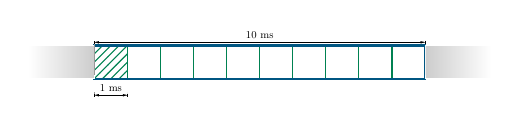
\begin{tikzpicture}[scale=.42, transform shape]
        \foreach \a in {0,1,...,9}{
            \draw[draw=KYJade] (\a,0) rectangle (1+\a,1);
        }
        \draw[pattern=north east lines, pattern color=KYJade,draw=KYJade] (0,0) rectangle (1,1);
        \draw[thick,draw=VCobalt] (0,0) rectangle (10,1);
        \draw[draw=white,left color=gray!40, right color=white] (10,0) rectangle (12,1);
        \draw[draw=white,right color=gray!40, left color=white] (-2,0) rectangle (0,1);
        \dimline[label style={anchor=south,font=\small,fill=white,text opacity=1,fill opacity=0},line style = {line width=.2 ,arrows=dimline-dimline},extension start length=.1,
extension end length=.1]{(0,1.1)}{(10,1.1)}{$10$ ms};         
        \dimline[label style={anchor=south,font=\small,fill=white,text opacity=1,fill opacity=0},line style = {line width=.2 ,arrows=dimline-dimline},extension start length=.1,
extension end length=.1]{(1,-.5)}{(0,-.5)}{$1$ ms};         
         \end{tikzpicture}
}
    \subfigure[1 Subframes = $2^\mu$ slots]{
        
\begin{tikzpicture}[scale=.42, transform shape]
        \foreach \a in {0,1,...,8}{
            \draw[draw=TAMustard] (\a,0) rectangle (1+\a,1);
        }
        \draw[pattern=north east lines, pattern color=TAMustard,draw=TAMustard] (0,0) rectangle (1,1);
        \draw[thick,draw=KYJade] (0,0) rectangle (8,1);
        \draw[draw=white,left color=VCobalt!40, right color=white] (8,0) rectangle (12,1);
        \draw[draw=white,right color=VCobalt!40, left color=white] (-4,0) rectangle (0,1);
        \dimline[label style={anchor=south,font=\small,fill=white,text opacity=1,fill opacity=0},line style = {line width=.2 ,arrows=dimline-dimline},extension start length=.1,
extension end length=.1]{(0,1.1)}{(8,1.1)}{$1$ ms};         
        \dimline[label style={anchor=south,font=\small,fill=white,text opacity=1,fill opacity=0},line style = {line width=.2 ,arrows=dimline-dimline},extension start length=.1,
extension end length=.1]{(1,-.75)}{(0,-.75)}{$\frac{1}{2^{\mu}}$ ms};         
         \end{tikzpicture}
}
    \subfigure[1 slot = 14 OFDM Symbols]{
        
\begin{tikzpicture}[scale=.42, transform shape]
        \foreach \a in {0,1,...,13}{
            \draw[draw=TZTeal] (.5*\a,0) rectangle (.5+.5*\a,1);
        }
        \draw[pattern=north east lines, pattern color=TZTeal,draw=TZTeal] (0,0) rectangle (.5,1);
        \draw[thick,draw=TAMustard] (0,0) rectangle (7,1);
        \draw[draw=white,left color=TAMustard!40, right color=white] (7,0) rectangle (11,1);
        \draw[draw=white,right color=TAMustard!40, left color=white] (-4,0) rectangle (0,1);
        \dimline[label style={anchor=south,font=\small,fill=white,text opacity=1,fill opacity=0},line style = {line width=.2 ,arrows=dimline-dimline},extension start length=.1,
extension end length=.1]{(0,1.1)}{(7,1.1)}{$\frac{1}{2^{\mu}}$ ms};         
        \dimline[label style={anchor=south,font=\small,fill=white,text opacity=1,fill opacity=0},line style = {line width=.2 ,arrows=dimline-dimline},extension start length=.1,
extension end length=.1]{(1,-.75)}{(0,-.75)}{$\frac{1}{14\cdot 2^{\mu}}$ ms};         
         \end{tikzpicture}
}
    \subfigure[OFDM $K =\frac{B}{2^{\mu} \Delta f_{ref}} \leq 4096$]{
        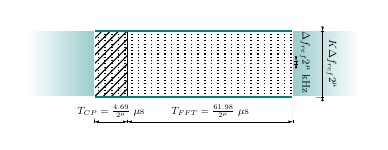
\begin{tikzpicture}[scale=.42, transform shape]
        \foreach \a in {0,1,...,19}{
            \draw[dotted] (0,0+.1*\a) rectangle (6,.1+.1*\a);
        }
        \draw[pattern=north east lines] (0,0) rectangle (1,2);
        \draw[thick,draw=TZTeal] (0,0) rectangle (6,2);
        \draw[draw=white,left color=TZTeal!40, right color=white] (6,0) rectangle (8,2);
        \draw[draw=white,right color=TZTeal!40, left color=white] (-2,0) rectangle (0,2);
        \dimline[label style={anchor=south,font=\small,fill=white,text opacity=1,fill opacity=0},line style = {line width=.2 ,arrows=dimline-dimline},extension start length=.1,
extension end length=.1]{(1,-.75)}{(0,-.75)}{$T_{CP}=\frac{4.69}{2^{\mu}}$ $\mu$s};       
        \dimline[label style={anchor=south,font=\small,fill=white,text opacity=1,fill opacity=0},line style = {line width=.2 ,arrows=dimline-dimline},extension start length=.1,
extension end length=.1]{(6,-.75)}{(1,-.75)}{$T_{FFT}=\frac{61.98}{2^{\mu}}$ $\mu$s};       
        \dimline[label style={anchor=south,font=\small,fill=white,text opacity=1,fill opacity=0},line style = {line width=.2 ,arrows=dimline reverse-dimline reverse},extension start length=.1,
extension end length=.1]{(6.1,1.1)}{(6.1,1.0)}{$\Delta f_{ref}2^{\mu}$ kHz};             
        \dimline[label style={anchor=south,font=\small,fill=white,text opacity=1,fill opacity=0},line style = {line width=.2 ,arrows=dimline reverse-dimline reverse},extension start length=.1,
extension end length=.1]{(6.9,2.0)}{(6.9,0)}{$K \Delta f_{ref} 2^{\mu}$};             
         \end{tikzpicture}
}
%         \caption{5G Radio Resources}
    \end{figure}  
 \end{column}
 \begin{column}{6cm}
 \begin{itemize}
  \item Cell discovery, synchronization, roaming etc. every \textit{several} frames\\ \ \\
  \item All numerologies co-exist in each subframe\\ \ \\
  \item Antenna Port Number: Limited Feedback Beamforming\\ \ \\
  \item De-Modulation Reference Signal (DMRS) every slot\\ \ \\
  \item Scheduler resolution mini-slot (2 OFDM sym. DMRS+data)\\ \ \\
 \end{itemize}
 \end{column}
\end{columns}  
}


\frame{
\frametitle{OFDM with Flexible Numerology}


    \begin{figure}
        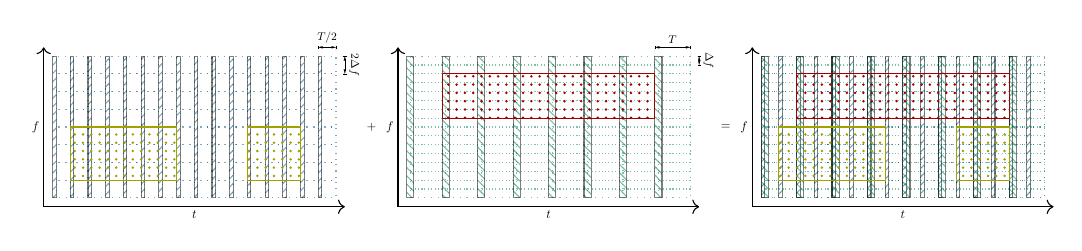
\begin{tikzpicture}[scale=.45, transform shape] 
            \foreach \x in {0,...,15}
        {
            \draw[pattern=north east lines,pattern color=VCobalt,opacity=.5] (0+.5*\x , 0) rectangle (.5*\x+.1,4);
            \foreach \y in {0,...,7}
            {  
                \draw[dotted,VCobalt,opacity=.5] (.1+.5*\x , .5*\y) rectangle (.5*\x+.5,.5*\y+.5);
            }
        }        
        \draw[pattern=dots,pattern color=TAMustard,draw=TAMustard] (.5 , .5) rectangle (3.5,2);
        \draw[pattern=dots,pattern color=TAMustard,draw=TAMustard] (5.5 , .5) rectangle (7,2);
        \draw[->] (-.25,-.25) -- node[anchor=north]{$t$} (8.25,-.25); 
        \draw[->] (-.25,-.25) -- node[anchor=east]{$f$} (-.25,4.25); 
        \dimline[label style={anchor=south,font=\small,fill=white,text opacity=1,fill opacity=0},line style = {line width=.2 ,arrows=dimline-dimline},extension start length=.25,
extension end length=.25]{(7.5,4.25)}{(8,4.25)}{$T/2$}; 
        \dimline[label style={anchor=south,font=\small,fill=white,text opacity=1,fill opacity=0},line style = {line width=.2 ,arrows=dimline-dimline},extension start length=.25,
extension end length=.25]{(8.25,4)}{(8.25,3.5)}{$2\Delta f$};
        \node at (9,2) {$+$};
            \foreach \x in {0,...,7}
        {
            \draw[pattern=north west lines,pattern color=KYJade,opacity=.5] (10+\x , 0) rectangle (\x+10.2,4);
            \foreach \y in {0,...,15}
            {
            \draw[dotted,KYJade,opacity=.5] (10.1+\x , .25*\y) rectangle (11+\x,.25+.25*\y);
            }
        }
        \dimline[label style={anchor=south,font=\small,fill=white,text opacity=1,fill opacity=0},line style = {line width=.2 ,arrows=dimline-dimline},extension start length=.25,
extension end length=.25]{(17,4.25)}{(18,4.25)}{$T$}; 
        \dimline[label style={anchor=south,font=\small,fill=white,text opacity=1,fill opacity=0},line style = {line width=.2 ,arrows=dimline-dimline},extension start length=.25,
extension end length=.25]{(18.25,4)}{(18.25,3.75)}{$\Delta f$};
        \draw[pattern=dots,pattern color=ARust,draw=ARust] (11 , 2.25) rectangle (17,3.5);
        \draw[->] (10-.25,-.25) -- node[anchor=north]{$t$} (10+8.25,-.25); 
        \draw[->] (10-.25,-.25) -- node[anchor=east]{$f$} (10-.25,4.25); 
        \node at (19,2) {$=$};
            \foreach \x in {0,...,15}
        {
            \draw[pattern=north east lines,pattern color=VCobalt,opacity=.5] (20+.5*\x , 0) rectangle (.5*\x+20.1,4);
            \foreach \y in {0,...,7}
            {  
                \draw[dotted,VCobalt,opacity=.5] (20.1+.5*\x , .5*\y) rectangle (.5*\x+20.5,.5*\y+.5);
            }
        }      
            \foreach \x in {0,...,7}
        {
            \draw[pattern=north west lines,pattern color=KYJade,opacity=.5] (20+\x , 0) rectangle (\x+20.2,4);
            \foreach \y in {0,...,15}
            {
            \draw[dotted,KYJade,opacity=.5] (20.1+\x , .25*\y) rectangle (21+\x,.25+.25*\y);
            }
        }
        \draw[pattern=dots,pattern color=TAMustard,draw=TAMustard] (20.5 , .5) rectangle (23.5,2);
        \draw[pattern=dots,pattern color=TAMustard,draw=TAMustard] (25.5 , .5) rectangle (27,2);
        \draw[pattern=dots,pattern color=ARust,draw=ARust] (21 , 2.25) rectangle (27,3.5);
        \draw[->] (20-.25,-.25) -- node[anchor=north]{$t$} (20+8.25,-.25); 
        \draw[->] (20-.25,-.25) -- node[anchor=east]{$f$} (20-.25,4.25); 
        \end{tikzpicture}
    \end{figure}
\begin{itemize}
 \item Multiple OFDM grids of different $\Delta f=\frac{1}{T}$ defined \textit{simultaneously}\\ \ \\
 \item Simultaneous data symbols assigned in either OFDM pattern\\ \ \\
 \item RF signal is sum of all component grids\\ \ \\
 \item \textbf{Flexible-size} orthogonal spectrum allocations\\ \ \\
 \item 5G \textbf{numerology} parameter $\mu=0,1,2\dots$, $\Delta f= 2^\mu \times 15kHz$
\end{itemize}
}


\frame[allowframebreaks]{\frametitle{Single Carrier OFDM}
\vspace{-.2in}
\begin{columns}[b]
 \begin{column}{6cm}  
        \begin{figure}    
    \subfigure[DAC Circuit]{
    \begin{tikzpicture}[auto, node distance=2cm,>=latex',scale=.3, transform shape]    
        \node [pinstyle] (xin) {x[n]};
        \node[block,right of=xin] (pul) {$p(t)$};
        \draw[->] (xin) -- (pul);
        \node[pinstyle, right of=pul] (xout) {$x(t)$};
        \draw[->] (pul) -- (xout);
        \node[coordinate, right of=xout,node distance=.6cm] (graphcoord) {};
        \begin{axis}[%
                    at={(graphcoord)},
                    width=8cm,
                    height=4cm,
                    axis x line=middle,
                    axis y line=middle,
                    xmax=8,
                    xmin=-1,
                    ymax=1.25,
                    ymin=-.25,
                    xlabel={$n$},
                    xticklabels={},
                    ylabel={$x(t)$},
                    yticklabels={},
                    x label style={at={(current axis.right of origin)},anchor=north west},
                    y label style={at={(current axis.above origin)},rotate=90,anchor= east},    
                    declare function={
                        sinc(\x)=(abs(\x)<0.01) ? 1 : (sin(180*\x)/(pi*\x)); % Definición de la función sinc(x)
                        }
                    ],
                    \addplot+[ARust,no marks,dashed,thick,domain = 0:7,samples=100] {sinc(x/2)};
                    \addplot+[ycomb,VCobalt,mark options={fill=VCobalt},thick,domain = 0:7,samples=8] {sinc(x/2)};
                \end{axis}
    \end{tikzpicture}
    }
    \\
    \subfigure[Waveform]{
            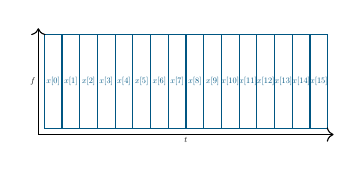
\begin{tikzpicture}[scale=.3, transform shape]
        \foreach \x in {0,...,15}
            {
                \draw[VCobalt] (\x*3/4,0) rectangle (\x*3/4+3/4,4) node[pos=.5] {$x[\x]$};
            }
        \draw[->] (-.25,-.25) -- node[anchor=north]{$t$} (12.25,-.25); 
        \draw[->] (-.25,-.25) -- node[anchor=east]{$f$} (-.25,4.25); 
        \end{tikzpicture}
    }
        \caption{Time Domain modulation}
    \end{figure}
 \end{column}
 \begin{column}{6cm}
    \begin{figure}
    \subfigure[DMT Circuit]{
    \begin{tikzpicture}[auto, node distance=2cm,>=latex',scale=.3, transform shape]    
        \node [pinstyle] (x0)  {$X^{(b)}[0]$};
        \foreach \a [evaluate=\a as \prev using int(\a-1)] in {1,2,...,7}{
            \node [pinstyle,below of=x\prev, node distance=.75cm] (x\a)  {$X^{(b)}[\a]$};
        }
        \node [coordinate, name=split] at ($(x3)!.5!(x4)-(1.25,0)$) {};
        \foreach \a in {0,1,...,7}{
            \draw [draw,->,align=center] (split) |- (x\a);
            }
        \node [block, left of=split,node distance=.75cm] (sp) {S/P};
        \draw [draw,-,align=center] (sp) -- (split);
        \node [pinstyle,left of=sp,node distance=1.5cm] (xin) {};
        \draw [draw,->,align=center] (xin) -- (sp);
        
        \node[block,minimum height=6cm] at ($(x3)!.5!(x4)+(2,0)$) (fft) {$8$-IFFT};
        \foreach \a in {0,1,...,7}{
            \node[coordinate] (inf\a) at ($(x\a)+(1.25,0)$) {};
            \draw[->] (x\a)--(inf\a);
        }
        \node[block,TAMustard,right of=fft] (pref) {CP};
        \draw[->] (fft) -- (pref);
        \node[block,right of=pref] (pul) {$p(t)$};
        \draw[->] (pref) -- node{$x[n]$} (pul);
        \node[pinstyle, right of=pul,node distance=1.5cm] (xout) {$x(t)$};
        \draw[->] (pul) -- (xout);
    \end{tikzpicture}
    }
    \\
    \subfigure[Waveform]{
        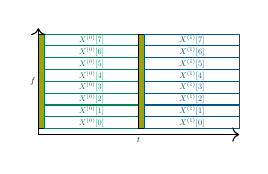
\begin{tikzpicture}[scale=.3, transform shape] 
            \draw[fill=TAMustard] (-.25,0) rectangle (0,4);
        \foreach \x in {0,...,7}
            {
                \draw[KYJade] (0,{\x/2}) rectangle (4,{(\x+1)/2}) node[pos=.5] {$X^{(0)}[\x]$};
            }
            \draw[fill=TAMustard] (4,0) rectangle (4.25,4);
        \foreach \x in {0,...,7}
            {
                \draw[VCobalt] (4.25,{\x/2}) rectangle (8.25,{(\x+1)/2}) node[pos=.5] {$X^{(1)}[\x]$};
            }
        \draw[->] (-.25,-.25) -- node[anchor=north]{$t$} (8.25,-.25); 
        \draw[->] (-.25,-.25) -- node[anchor=east]{$f$} (-.25,4.25); 
        \end{tikzpicture}
        }
        \caption{OFDM modulation}
    \end{figure}
   \end{column} 
\end{columns}
\begin{itemize}
 \item OFDM very high Peak To Average Power Ratio (PAPR)
\end{itemize}

\begin{columns}[b]
 \begin{column}{6cm}  
    \begin{figure}
    \subfigure[Circuit]{
    \begin{tikzpicture}[auto, node distance=2cm,>=latex',scale=.3, transform shape]    
        \node [pinstyle] (x0)  {$X^{(b)}[0]$};
        \foreach \a [evaluate=\a as \prev using int(\a-1)] in {1,2,...,7}{
            \node [pinstyle,below of=x\prev, node distance=.75cm] (x\a)  {$X^{(b)}[\a]$};
        }
        \node [block,minimum height=3cm] at ($(x1)!.5!(x2)-(2,0)$) (scfft0) {$4$-FFT};
        \node [block,minimum height=3cm,opacity=.5] at ($(x5)!.5!(x6)-(2,0)$) (scfft1) {$4$-FFT};
        \node [coordinate, name=split]  at ($(scfft0)!.5!(scfft1)-(3.5,0)$) {};
        \foreach \b in {0,1}
        {
            \foreach \c [evaluate=\c as \a using int(\c+4*\b)] in {0,1,...,3}{
                \node[coordinate] (inf\a) at ($(x\a)-(1.25,0)$) {};
                \draw [draw,->,align=center,opacity={1/(1+\b)}] (inf\a) -- (x\a);
                \node[pinstyle,opacity={1/(1+\b)}] (xsc\a) at ($(inf\a)-(2.75,0)$) {$X_{SC}^{(b)}[\b,\c]$};
                \node[coordinate] (aux\a) at ($(inf\a)-(1.5,0)$) {};
                \draw [draw,->,align=center,opacity={1/(1+\b)}] (split) |- (xsc\a);
                \draw [draw,->,align=center,opacity={1/(1+\b)}] (xsc\a) -- (aux\a);
                }                
        }
        \node [block, left of=split,node distance=.75cm] (sp) {S/P};
        \draw [draw,-,align=center] (sp) -- (split);
        \node [pinstyle,left of=sp,node distance=1.5cm] (xin) {};
        \draw [draw,->,align=center] (xin) -- (sp);
        
        \node[block,minimum height=6cm] at ($(x3)!.5!(x4)+(2,0)$) (fft) {$8$-IFFT};
        \foreach \a in {0,1,...,7}{
            \node[coordinate] (inf\a) at ($(x\a)+(1.25,0)$) {};
            \draw[->] (x\a)--(inf\a);
        }
        \node[pinstyle, right of=fft,node distance=1.75cm] (xout) {$\dots$};
        \draw[->] (fft) -- (xout);
    \end{tikzpicture}
    }
    \\
    \subfigure[Waveform]{   
        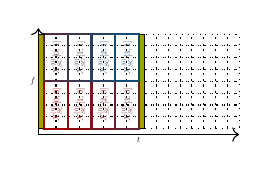
\begin{tikzpicture}[scale=.3, transform shape] 
        \draw[fill=TAMustard] (-.25,0) rectangle (0,4);  
        \draw[fill=TAMustard] (4,0) rectangle (4.25,4);        
        \foreach \y in {0,...,7}
        {
            \foreach \x in {0,...,7}
            {
            \draw[dotted] (.5*\x , .5*\y) rectangle (.5*\x+.5,.5*\y+.5);
            \draw[dotted] (4.25+.5*\x , .5*\y) rectangle (4.25+.5*\x+.5,.5*\y+.5);
            }
        }
        
        \foreach \b in {0,1}
        {
            \foreach \c in {0,1,...,3}{
                \pgfmathsetmacro\colorinfor{\b*50+\c*12.5}
                \draw[VCobalt!\colorinfor!ARust,thick] (0+\c,0+2*\b) rectangle (1+\c,2+2*\b);
                \node[VCobalt!\colorinfor!ARust,rotate=90] at (\c+.5,2*\b+1) {$X_{SC}^{(0)}[\c,\b]$};
            }
        }
        \draw[->] (-.25,-.25) -- node[anchor=north]{$t$} (8.25,-.25); 
        \draw[->] (-.25,-.25) -- node[anchor=east]{$f$} (-.25,4.25); 
        \end{tikzpicture}
        }
        \caption{Contiguous SC-OFDM}
    \end{figure}
   \end{column} 
 \begin{column}{6cm}  
    \begin{figure}
    \subfigure[Circuit]{
    \begin{tikzpicture}[auto, node distance=2cm,>=latex',scale=.3, transform shape]    
        \node [pinstyle] (x0)  {$X^{(b)}[0]$};
        \foreach \a [evaluate=\a as \prev using int(\a-1)] in {1,2,...,7}{
            \node [pinstyle,below of=x\prev, node distance=.75cm] (x\a)  {$X^{(b)}[\a]$};
        }
        \node [block,minimum height=3cm] at ($(x1)!.5!(x2)-(4,0)$) (scfft0) {$4$-FFT};
        \node [block,minimum height=3cm,opacity=.5] at ($(x5)!.5!(x6)-(4,0)$) (scfft1) {$4$-FFT};
        \foreach \b in {0,1}
        {
            \foreach \c [evaluate=\c as \a using int(\c+4*\b)] in {0,1,...,3}{
                \node[coordinate] (inf\a) at ($(x\a)-(3.25,0)$) {};
                \node[coordinate] (inter\a) at ($(x\a)-(1.25,0)$) {};
                \node[coordinate] (aux\a) at ($(inf\a)-(1.5,0)$) {};
                \node[pinstyle,left of=aux\a,opacity={1/(1+\b)}] (xsc\a) {$X_{SC}^{(b)}[\b,\c]$};
                \draw [draw,->,align=center,opacity={1/(1+\b)}] (xsc\a) -- (aux\a);
                }                
        }
        \foreach \b in {0,1}
        {
            \foreach \c [evaluate=\c as \a using int(\c+4*\b),evaluate=\c as \d using int(2*\c+\b)] in {0,1,...,3}{
                \draw [draw,align=center,opacity={1/(1+\b)}] (inf\a) -- (inter\d);
                \draw [draw,->,align=center,opacity={1/(1+\b)}] (inter\d) -- (x\d);
                }                
        }
        
        \node[block,minimum height=6cm] at ($(x3)!.5!(x4)+(2,0)$) (fft) {$8$-IFFT};
        \foreach \a in {0,1,...,7}{
            \node[coordinate] (inf\a) at ($(x\a)+(1.25,0)$) {};
            \draw[->] (x\a)--(inf\a);
        }
        \node[pinstyle, right of=fft,node distance=1.75cm] (xout) {$\dots$};
        \draw[->] (fft) -- (xout);
    \end{tikzpicture}
    }
    \\
    \subfigure[Waveform]{   
        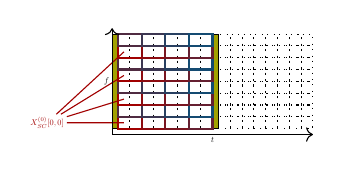
\begin{tikzpicture}[scale=.3, transform shape] 
        \draw[fill=TAMustard] (-.25,0) rectangle (0,4);  
        \draw[fill=TAMustard] (4,0) rectangle (4.25,4);        
        \foreach \y in {0,...,7}
        {
            \foreach \x in {0,...,7}
            {
            \draw[dotted] (.5*\x , .5*\y) rectangle (.5*\x+.5,.5*\y+.5);
            \draw[dotted] (4.25+.5*\x , .5*\y) rectangle (4.25+.5*\x+.5,.5*\y+.5);
            }
        }
        
        \foreach \a in {0,1,...,3}
        {
            \foreach \b in {0,1}
            {
                \foreach \c in {0,1,...,3}{
                    \pgfmathsetmacro\colorinfor{\b*50+\c*12.5}
                    \draw[VCobalt!\colorinfor!ARust,thick] (0+\c,0+\a+\b/2) rectangle (1+\c,.5+\a+\b/2);
                }
            }
        }
        \node[ARust] (number) at (-3,.25) {$X_{SC}^{(0)}[0,0]$};
        \foreach \a in {0,1,...,3}
        {
            \draw[ARust] (.25,.25+\a) -- (number);
        }
        \draw[->] (-.25,-.25) -- node[anchor=north]{$t$} (8.25,-.25); 

        \draw[->] (-.25,-.25) -- node[anchor=east]{$f$} (-.25,4.25); 
        \end{tikzpicture}
        }
        \caption{Interleaved SC-OFDM}
    \end{figure}
   \end{column} 
\end{columns}

\begin{itemize}
 \item Mandatory LTE Uplink, optional ``Transform precoding'' in 5G
\end{itemize}


}
\frame[allowframebreaks]{
\frametitle{Orthogonal Time Frequency Space (OTFS)}
\begin{itemize}
 \item Time-variant CIR $h(\tau,t_o)$
 \item Periodogram transfer function $H[k](t_o)$
 \item Scattering function $S_h(\tau,\nu)$
 \item Fourier transform $H(f,\nu)$
 \begin{itemize}
  \item 2-path example $H[k](t_o)=1+e^{-j2\pi \frac{k t_o\nu_1}{K}}$
 \end{itemize} 
\end{itemize}
\begin{columns}
 \begin{column}{6cm}
 \begin{figure}
 \centering
 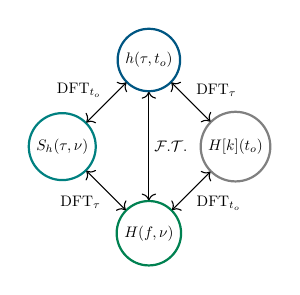
\begin{tikzpicture}[scale=.55, transform shape] 
        \node[circle,draw=VCobalt,thick,minimum size=1.2cm] (t) at (0,0) {$h(\tau,t_o)$};   
        \node[circle,draw=gray,thick,minimum size=1.2cm] (tf) at (2,-2) {$H[k](t_o)$};
        \node[circle,draw=TZTeal,thick,minimum size=1.2cm] (dd) at (-2,-2) {$S_h(\tau,\nu)$};
        \node[circle,draw=KYJade,thick,minimum size=1.2cm] (f) at (0,-4) {$H(f,\nu)$};
        \draw[<->] (t)-- node[anchor=south east]{$\mathrm{DFT}_{t_o}$} (dd); 
        \draw[<->] (f)-- node[anchor=north east]{$\mathrm{DFT}_{\tau}$} (dd); 
        \draw[<->] (tf)-- node[anchor=north west]{$\mathrm{DFT}_{t_o}$} (f); 
        \draw[<->] (t)-- node[anchor=south west]{$\mathrm{DFT}_{\tau}$} (tf); 
        \draw[<->] (t)-- node[anchor=west]{$\mathcal{F.T.}$} (f); 
%         \draw [->] (t) to [out=-70,in=70] node[anchor=south,rotate=-90]{Wigner} (tf);
%         \draw [->] (tf) to [out=110,in=-110] node[anchor=south,rotate=90]{Heisenberg} (t);
        \end{tikzpicture}
 \caption{Time-varying transforms}
\end{figure}    
 \end{column}
 \begin{column}{6cm}
 \begin{figure}
 \centering
 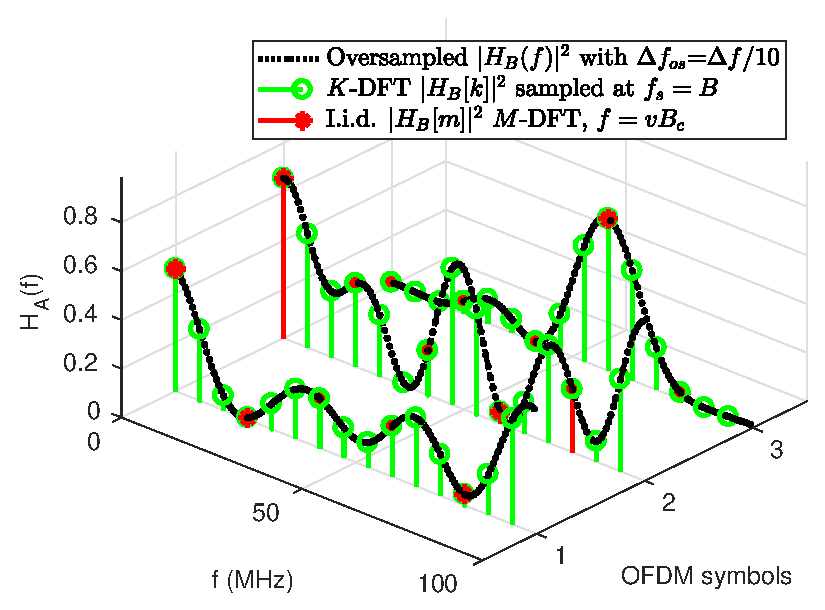
\includegraphics[width=.9\columnwidth]{DFTHBD}
 \caption{T.V. 2-path OFDM channel}
\end{figure}    
 \end{column}
\end{columns}

\pagebreak

\begin{definition}[Zak Transform of $x(t)$ with parameter $T$]
$$Z_x(\tau,\nu)=\sum_{v=-\infty}^{\infty}x(v\tau+t)e^{-j2\pi\nu (t-\tau)}\forall \tau\in[0,T),\nu\in[-\frac{1}{2T},\frac{1}{2T})$$
\end{definition}
 \begin{figure}
 \subfigure[Periodogram]{
        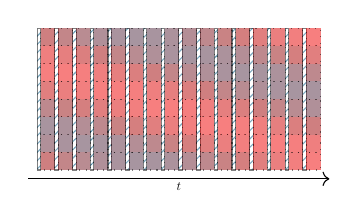
\begin{tikzpicture}[scale=.45, transform shape] 
            \foreach \x in {0,...,15}
        {
            \draw[pattern=north east lines,pattern color=VCobalt,opacity=.5] (0+.5*\x , 0) rectangle (.5*\x+.1,4);
            \foreach \y in {0,...,7}
            {  
                \pgfmathsetmacro\colorinfor{.5+.5*sin(360*(\y+\x/3)/7)*100}
                \draw[dotted,fill=VCobalt!\colorinfor!ARust,opacity=.5] (.1+.5*\x , .5*\y) rectangle (.5*\x+.5,.5*\y+.5);
            }
        }        
        \draw[->] (-.25,-.25) -- node[anchor=north]{$t$} (8.25,-.25); 
        \end{tikzpicture}
        }
 \subfigure[Zak Transform]{
 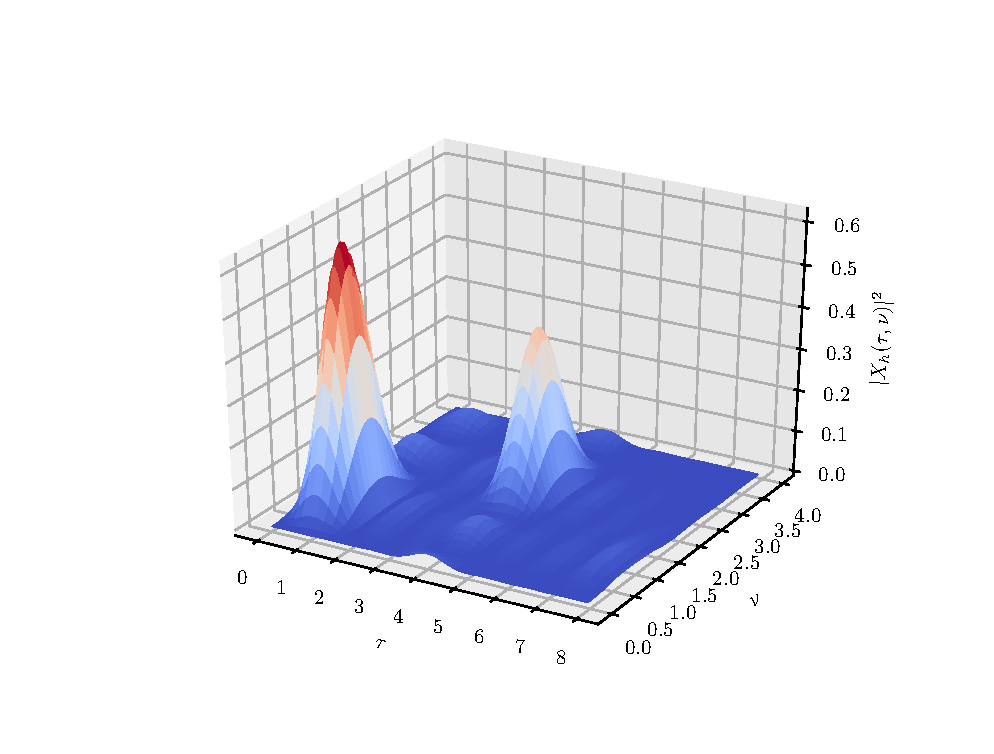
\includegraphics[trim={1cm 1cm 1cm 1cm},clip,width=.36\columnwidth]{2pathchanexample}
        }
%         \caption{Z}
    \end{figure}  
    
    \pagebreak
    
\begin{columns}[T]
 \begin{column}{8cm}
 
\begin{definition}[DZT - OTFS Modulation]
Sampling $t=nT_s$, $D=T/T_s$, $n=d+vD$
$$Z_x[d,v]=\sum_{u=0}^{V-1}x[vD+d]e^{-j2\pi\frac{uv}{V}}\forall x[n]\textnormal{ with period }L=VD$$
\vspace{-.3in}
    \begin{figure}    
    \subfigure[4-2-DZT symbols at TF grid]{
        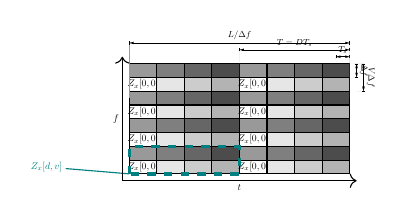
\begin{tikzpicture}[scale=.35, transform shape] 
        \foreach \x in {0,1}
        \foreach \y in {0,...,3}
        {
            \foreach \a in {0,...,3}
            \foreach \b in {0,...,1}
                {
                    \draw[fill=black, fill opacity={(\a+4*\b)/10}] (4*\x+\a     ,{\y+\b/2}) rectangle (4*\x+\a+1,{(\y+\b/2+1/2)});
                }
                
            \node at (4*\x+.5,\y+1/4) {$Z_x[0,0]$};
        }
        \dimline[label style={anchor=south,font=\small,fill=white,text opacity=1,fill opacity=0},line style = {line width=.2 ,arrows=dimline-dimline},extension start length=.25,
extension end length=.25]{(7.5,4.25)}{(8,4.25)}{$T_s$}; 
        \dimline[label style={anchor=south,font=\small,fill=white,text opacity=1,fill opacity=0},line style = {line width=.2 ,arrows=dimline-dimline},extension start length=.25,
extension end length=.25]{(4,4.5)}{(8,4.5)}{$T=DT_s$}; 
        \dimline[label style={anchor=south,font=\small,fill=white,text opacity=1,fill opacity=0},line style = {line width=.2 ,arrows=dimline-dimline},extension start length=.25,
extension end length=.25]{(0,4.75)}{(8,4.75)}{$L/\Delta f$}; 
        \dimline[label style={anchor=south,font=\small,fill=white,text opacity=1,fill opacity=0},line style = {line width=.2 ,arrows=dimline-dimline},extension start length=.25,
extension end length=.25]{(8.25,4)}{(8.25,3.5)}{$\Delta f$};
        \dimline[label style={anchor=south,font=\small,fill=white,text opacity=1,fill opacity=0},line style = {line width=.2 ,arrows=dimline-dimline},extension start length=.25,
extension end length=.25]{(8.5,4)}{(8.5,3)}{$V\Delta f$};
        \draw[TZTeal,very thick,dashed] (0,0) rectangle (4,1);
        \node[TZTeal] (number) at (-3,.25) {$Z_x[d,v]$};
        \draw[TZTeal] (0,0) -- (number);
        \draw[->] (-.25,-.25) -- node[anchor=north]{$t$} (8.25,-.25); 
        \draw[->] (-.25,-.25) -- node[anchor=east]{$f$} (-.25,4.25); 
        \end{tikzpicture}}
        \hspace{.05in}
        \subfigure[2-4-DZT FFTs]{
        \begin{tikzpicture}[scale=.35, transform shape,auto, node distance=1.5cm,>=latex']
        \foreach \x in {0,...,3}
            \foreach \y [evaluate={\z= int(2*\x+\y)}] in {0,1}
                {
                    \node (x\z) at ({2*\x+\y},0) {$x[\z]$} ;
                }
       \node[block,below of =x0,node distance=2cm, anchor=west,minimum width=3.4cm] (fft0) {$\frac{L}{D}$-FFT} ;
       \node[block,below of =x7,node distance=2cm, anchor=east,minimum width=3.4cm] (fft1) {$\frac{L}{D}$-FFT} ;
        \foreach \x in {0,...,3}
            \foreach \y [evaluate={\z= int(2*\x+\y)}] in {0,1}
                {
                    \draw[->] (x\z) -- ++(0,-.5) -- (fft\y);
                }
        
        \foreach \x in {0,...,3}
            \foreach \y [evaluate={\z= int(2*\x+\y)}] in {0,1}
                {
                    \node (Zx\z) at ({4*\y+\x},-4) {$Z_x^{[\y,\x]}$} ;
                }
        \foreach \x in {0,...,3}
            \foreach \y [evaluate={\z= int(2*\x+\y)}] in {0,1}
                {
                    \draw[<-] (Zx\z) -- ++(0,1.5);
                }
        \end{tikzpicture}
        }
    \caption{OTFS vs OFDM FFT}
\end{figure}
\vspace{-.1in}
% $$Z_y[d,v]=\sum_{u'=0}^{V-1}\sum_{d'=0}^{D-1}Z_h[d-d',v-v']Z_x[d',v']+Z_r[d,v]$$
\end{definition}
 \end{column}
 \begin{column}{4cm}
\begin{figure}[t]
 \centering 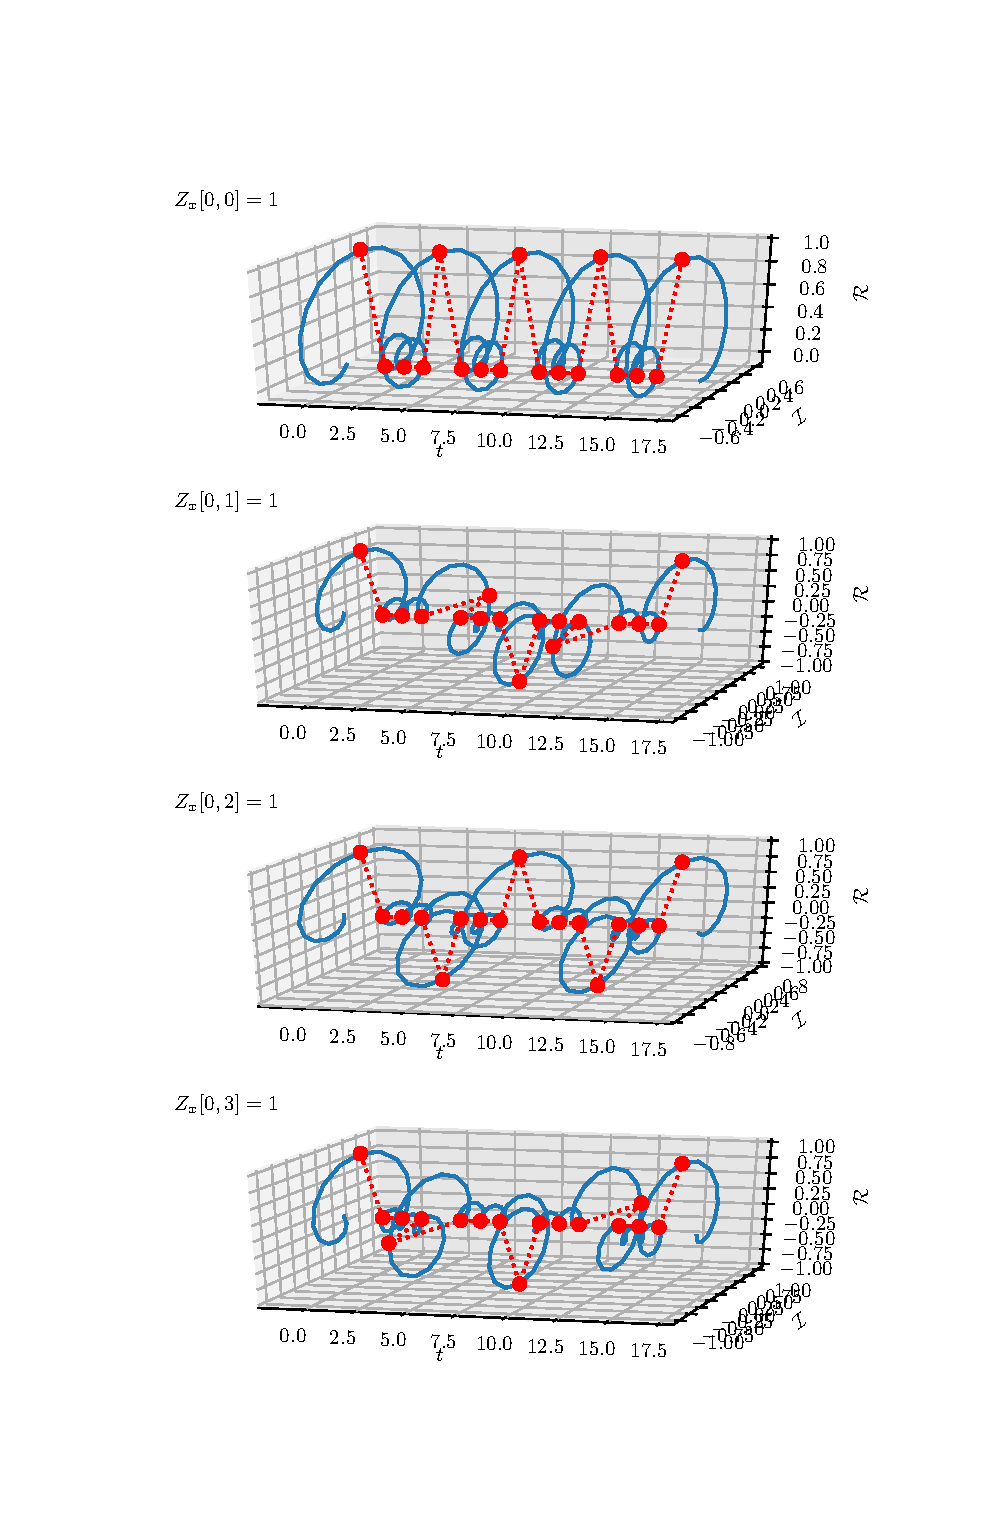
\includegraphics[trim={1cm 2.5cm 1cm 2.5cm},clip,width=\columnwidth]{pulses3D}
 \caption{OTFS Orthonormal Pulses}
 \vspace{-.2in}
\end{figure}  
 \end{column}
\end{columns}  
}



\end{document}


